% Initial manuscript for IFAC INCOM 2027.
% Official class and bibliography style were downloaded on 2026-07-13.
\pdfminorversion=4
\documentclass{ifacconf}

\usepackage{graphicx}
\usepackage{natbib}
\usepackage{booktabs}
\usepackage{amsmath,amssymb}
\usepackage{array}

\begin{document}
\begin{frontmatter}

\title{Structure-Aware Optimization for Dual-Source Rotary Cluster-Tool Scheduling}

\author[inst]{Author Name}
\address[inst]{Affiliation, City, Country (e-mail: author@example.com).}

\begin{abstract}
Product wafers and reusable process-enabling carriers enter a rotary cluster tool from different stores but compete for the same robots, load locks, and chambers. We formulate their finite-horizon scheduling problem with serial alignment, loaded and empty robot motion, two rotary recipes, carrier reuse, and cleaning. A structure-preserving binary-skeleton warm start supplies feasible incumbents without restricting the original mixed-integer model. A role-aware selector then ranks solver-generated cutting planes. Exact validation exposes the mixed-recipe computational bottleneck and defines a paired evaluation against SCIP, Adaptive Cut Selection, and HEM.
\end{abstract}

\begin{keyword}
Production scheduling; semiconductor manufacturing; mixed-integer programming; cluster tools; cutting planes; machine learning.
\end{keyword}

\end{frontmatter}

\section{Introduction}

The throughput of a semiconductor cluster tool depends on decisions that are easy to omit from an aggregate chamber schedule. A wafer must be picked from the correct source, aligned, assigned to a load-lock slot, transported by an available robot, exposed on the correct chamber side, and returned. Empty robot repositioning is equally physical: two loaded moves cannot be consecutive when the second pick starts at the previous destination. These details become more consequential when product wafers share the equipment with reusable process-enabling carrier (PEC) wafers.

We study a dual-source rotary tool with an atmospheric robot (ATR), a single-slot aligner (AL), upper and lower load locks (LL), a vacuum robot (VTR), and two four-pocket rotary chambers. Product wafers start and finish at load ports, whereas PEC wafers start and finish at a dedicated store. The tool supports a four-wafer recipe ($4\times1$) and a pair-exchange recipe ($2\times2$). Cleaning is a pure-PEC rotary batch. The operational objective is the completion time of the last returned product wafer.

Recent cluster-tool studies address non-cyclic schedules, concurrent wafer types, and residency constraints through mathematical programming or learned dispatching \citep{ahn2025cluster,kim2025adaptive,li2025cyclic,yang2025residency}. The present equipment adds a reusable auxiliary material stream, two incompatible rotary grammars, and cleaning that may interrupt a pair-exchange chain. The resulting model is a difficult mixed discrete--continuous scheduling problem.

This paper develops three connected contributions. First, it gives a physically explicit mixed-integer formulation in which AL capacity, both loaded and empty robot motion, LL slots, PEC conservation, rotary-side exposure, and cleaning are decision constraints rather than post-processing checks. Second, it introduces a structure-preserving binary-skeleton (SPBS) warm start that asks a temporary model to complete high-confidence recipe choices into a feasible incumbent; the original feasible region is unchanged. Third, it describes candidate cutting planes by the coefficient mass carried by solver-visible variable roles and combines hierarchical learned ordering with a role-coverage completion rule. The last component is domain independent even though the motivating model is a cluster tool.

\section{Related Work}

Cluster-tool scheduling has been studied under cyclic, non-cyclic, and multi-product operation. Precomputed cyclic schedules are attractive when the equipment repeats a stable recipe, but they do not directly cover a finite mixed lot with cleaning and a reusable auxiliary material stream. Precedence-based mixed-integer models improve the representation of non-cyclic robot moves \citep{ahn2025cluster}. Concurrent-processing studies additionally consider adaptive wafer release or learned robot actions \citep{kim2025adaptive}. Residency-constrained models show that apparently local waiting decisions can alter global feasibility \citep{li2025cyclic,yang2025residency}. Our formulation shares their emphasis on explicit timing, but focuses on rotary-side exchange and PEC conservation across two sources.

Learning inside exact optimization addresses a different layer. Rather than replacing a solver, a learned component can guide branching, primal heuristics, or separation decisions while preserving the mathematical model. Cut selection is suitable for a safety-preserving interface: the solver first generates valid inequalities, and the policy only decides which candidates enter the relaxation. Huang et al. learn candidate-level cut scores \citep{huang2022learning}; HEM couples retained cardinality with an ordered sequence \citep{wang2023hem}; Adaptive Cut Selection predicts or tunes the weights in SCIP's hybrid score \citep{turner2023adaptive}. These methods primarily describe immediate numerical quality. Our role features add whether row coefficients act on discrete choices, continuous timing variables, or both.

The warm start and cut selector have deliberately different domains. SPBS uses the known scheduling grammar and is meaningful only for this equipment family. The cut representation uses only variable type, objective coefficient, bounds, and row coefficients available through SCIP. Separating the claims prevents a successful scheduling heuristic from being presented as generic learning and prevents cross-family cut results from substituting for manufacturing validation.

\section{Equipment and Scheduling Logic}

\subsection{Two material sources and one-slot alignment}

Let $W=W^{F}\cup W^{M}$ contain the product wafers for the $4\times1$ and $2\times2$ recipes, $Q$ be the finite set of reusable PEC tokens, and $C$ be the two rotary chambers. A product wafer follows
\[
\begin{aligned}
\mathrm{LP}&\rightarrow\mathrm{ATR}\rightarrow\mathrm{AL}\rightarrow\mathrm{LL}^{up}
\rightarrow\mathrm{VTR}\rightarrow\mathrm{CH}\\
&\rightarrow\mathrm{LL}^{low}\rightarrow\mathrm{ATR}\rightarrow\mathrm{LP}.
\end{aligned}
\]
A PEC follows $\mathrm{PECStore}\rightarrow\mathrm{VTR}\rightarrow\mathrm{CH}\rightarrow\mathrm{VTR}\rightarrow\mathrm{PECStore}$. Because AL has one slot, two wafers held by ATR are calibrated serially. The model therefore contains place, calibrate, remove, and companion-place events; a fictitious two-wafer AL operation is not allowed.

Product wafers of the same recipe are paired. If only one product wafer remains, the load port releases that wafer alone and the missing chamber position is filled by a real PEC token. This rule prevents the ``empty wafer'' artifacts that arise when a fixed-size pair is created regardless of remaining demand.

\subsection{Rotary recipes and cleaning}

An active $4\times1$ batch loads a pair on each chamber side, processes the four occupied pockets, and unloads both sides after the required rotations. A tail side may contain PEC fillers. In the $2\times2$ recipe, product pairs form a contiguous exchange chain between a PEC head and a PEC tail. Each product pair participates in two adjacent exposures; the interval between those exposures is a necessary bridge wait used to exchange one pair.

After a configured number of full-chamber process cycles, cleaning is represented as a pure-PEC batch with the same VTR and rotary-side constraints as production. A $2\times2$ chain need not finish before cleaning. Instead, the triggering segment first converts the chamber contents to PEC, cleaning occupies the chamber, and a later PEC-bounded segment resumes product exchange. Pure-PEC chamber contents are consequently permitted at cleaning transitions, not as an ordinary production shortcut.

\section{Mixed-Integer Scheduling Model}

\subsection{Assignment and activation}

Let $P$ be the set of product pairs, $B_c$ the candidate $4\times1$ batches on chamber $c$, and $K_c$ the candidate $2\times2$ chain positions. Binary variables $x^F_{pbhc}$ and $x^M_{pkc}$ assign pair $p$ to side $h$ of a full batch or to an exchange position. Each pair is used once:
\begin{equation}
 \sum_{c\in C}\left(\sum_{b\in B_c}\sum_{h=1}^{2}x^F_{pbhc}
 +\sum_{k\in K_c}x^M_{pkc}\right)=1,\quad p\in P.
 \label{eq:assignment}
\end{equation}
Batch and position activation variables make used positions a contiguous prefix. Further binary variables select LL slots, cleaning epochs, and the order of optional tasks that share a unary resource.

\subsection{Time intervals and physical resources}

Each action $a$ has start $s_a$, completion $e_a$, and duration $d_a$. For two optional actions $a$ and $b$ on the same robot or module, an order variable $y_{ab}$ enforces
\begin{align}
s_b &\ge e_a+\delta_{ab}-M(1-y_{ab}),\nonumber\\
s_a &\ge e_b+\delta_{ba}-My_{ab},
\label{eq:resource}
\end{align}
where $\delta_{ab}$ is the endpoint-dependent empty repositioning time. The same construction coordinates ATR, VTR, AL, chamber windows, and explicit LL slots. Loaded travel, pickup, and placement are separate from the empty move to the next pickup location.

A PEC token is occupied from the start of its VTR chamber-bound load until its VTR unload has returned it to storage. Overlap constraints prevent the same token from supporting two chamber intervals. Rotary precedences couple front-side load, half rotation, rear-side load or exchange, exposure, unload, and the return rotation. The primary objective is
\begin{equation}
 \min C_{\max},\qquad C_{\max}\ge C^{\mathrm{return}}_w\quad(w\in W).
 \label{eq:makespan}
\end{equation}
An optional second solve fixes the optimal or best-known $C_{\max}$ and compacts avoidable waits for visualization. This lexicographic phase cannot sacrifice throughput for a smoother Gantt chart.

\subsection{Occupancy and flow invariants}

Resource non-overlap alone does not guarantee that a schedule respects material state. For each explicit LL slot $r$, an occupancy interval begins when ATR places a product wafer and ends when VTR removes it; the return direction is defined analogously. Optional intervals are activated only when their wafer uses slot $r$, and pairwise disjunctions prevent two active occupancies from overlapping. AL occupancy is modeled in the same way, but with one slot and serial precedences between paired wafers.

For each PEC token $q$, let $u_{q\ell}$ indicate assignment to chamber-support interval $\ell$. Token conservation requires
\begin{equation}
\begin{aligned}
 \sum_{q\in Q}u_{q\ell}&=n^{PEC}_{\ell},\\
 [S_{\ell},E_{\ell})\cap[S_{\ell'},E_{\ell'})&=\emptyset
 \quad\text{if }u_{q\ell}=u_{q\ell'}=1,
\end{aligned}
\label{eq:pec}
\end{equation}
where $n^{PEC}_{\ell}$ is the number of physical fillers required. The interval begins before chamber-bound pickup and ends after return placement, not merely at chamber exposure. Thus a token carried or waiting on VTR cannot be assigned elsewhere.

Recipe-state variables link chamber contents across rotations. A $4\times1$ tail indicator permits PEC on an unused side only after all earlier active production batches. For $2\times2$, predecessor and successor variables connect active exchange positions; no hole can appear inside a chain. Cleaning epoch variables split the chain into segments. The final exposure of a pre-clean segment must establish a pure-PEC chamber state, and the first post-clean segment starts from a PEC state. This is a transition invariant, not a general permission for an all-PEC production chamber.

Robot location is also a state. If task $a$ ends at location $v$ and the next loaded task $b$ picks at $u$, $\delta_{ab}$ in (\ref{eq:resource}) contains the allowed empty move $v\rightarrow u$. When $v=u$, it may be zero; otherwise it is positive. This prevents a Gantt lane from showing incompatible loaded moves without the intervening return. It also supports an unambiguous utilization decomposition: pickup/place and loaded/empty travel are busy, holding a wafer without motion is loaded waiting, and having no wafer and no action is idle.

\section{Structure-Aware Solution Strategy}

\subsection{Binary-skeleton warm start}

SPBS separates robust recipe logic from fragile timing choices. In a temporary copy of the scheduling model it fixes high-confidence assignment, batch activation, cleaning-epoch, and LL-slot binaries. Local ATR/AL/LL orders may also be fixed. VTR orders remain free in a relaxed fallback profile because they have large downstream effects. All continuous times and all unfixed resource orders are completed by SCIP. A feasible temporary solution is passed to the original model as an incumbent; if completion fails, the original solve simply starts without it. No bound or constraint is transferred.

For $4\times1$, the skeleton fills complete product batches and uses PEC only on a tail side. For $2\times2$, it creates PEC-bounded exchange segments and places a segment boundary at cleaning. This construction addresses the main feasibility failure observed with a naive policy that waits for an entire exchange chain before cleaning.

The operational sequence is: (1) construct canonical product pairs and identify the single-wafer tail; (2) allocate complete $4\times1$ batches and contiguous $2\times2$ segments; (3) insert a PEC-conversion boundary at each required cleaning epoch; (4) fix the selected binary profile in a temporary copy; (5) let SCIP complete all timing variables and unfixed orders under a short limit; and (6) verify and transfer a feasible solution to the original model. If the full profile fails, step 4 is repeated with VTR-order variables free. This fallback is important because a locally plausible VTR sequence can conflict with a chamber rotation several operations later.

\subsection{Role-aware cut selection}

SCIP generates valid candidate cuts and normally retains a subset \citep{bestuzheva2023scip}. Learned selectors rank individual candidates \citep{huang2022learning}, jointly predict cardinality and order \citep{wang2023hem}, or adapt SCIP's hybrid-score weights \citep{turner2023adaptive}. For a candidate row $i$, $\sum_j a_{ij}x_j\le b_i$, we augment the 13 generic HEM features with normalized coefficient mass
\begin{equation}
p_{ig}=\frac{\sum_{j:x_j\in g}|a_{ij}|}{\sum_j|a_{ij}|+\epsilon},
\quad g\in\{B,I,C_o,C_a,O\},
\label{eq:roles}
\end{equation}
for binary, general-integer, objective-active continuous, continuous auxiliary, and residual roles. Five role masses, bounded-variable mass, positive-coefficient mass, discrete--continuous coupling, dominant-role mass, and role entropy produce a 23-dimensional, name-invariant candidate vector.

\begin{table}[t]
\begin{center}
\caption{Role features appended to the 13 HEM features.}\label{tab:features}
\begin{tabular}{cl}
\toprule
Count & Description\\
\midrule
5 & Mass on $B,I,C_o,C_a,O$\\
1 & Mass on globally bounded variables\\
1 & Positive-coefficient mass\\
1 & Discrete--continuous coupling\\
1 & Dominant non-residual role mass\\
1 & Normalized role entropy\\
\bottomrule
\end{tabular}
\end{center}
\end{table}

The coupling feature is $4(p_{iB}+p_{iI})(p_{iC_o}+p_{iC_a})$; it is largest when a row balances discrete and continuous coefficient mass. Dominant mass distinguishes a focused row, while entropy distinguishes broad mixtures of roles. None of these definitions uses a variable name, route identifier, or constraint label. The feature schema is versioned so that checkpoints trained under an older 23-dimensional meaning cannot be loaded silently.

A hierarchical policy predicts the retained cardinality and an ordering. Its prefix anchors the decision. Remaining slots are filled greedily under a nonnegative sum of cut quality, concave role coverage, and facility-location representativeness. This completion objective is monotone submodular; for fixed anchors, cardinality-constrained greedy obtains the standard $1-1/e$ residual approximation \citep{nemhauser1978submodular}. Only SCIP-generated cuts are reordered, so integer feasibility is unaffected.

\begin{figure}[t]
\begin{center}
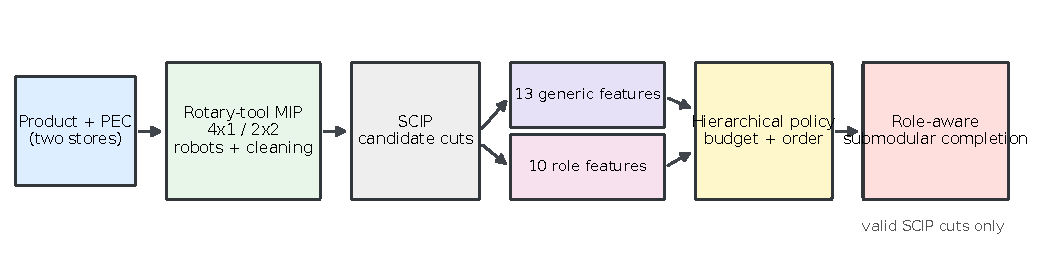
\includegraphics[width=8.35cm]{rdmct_pipeline.pdf}
\caption{Scheduling model, SCIP candidate cuts, hierarchical selection, and role-aware completion.}
\label{fig:pipeline}
\end{center}
\end{figure}

\section{Validation and Experimental Design}

\subsection{Current formulation evidence}

Table~\ref{tab:validation} reports deterministic connectivity checks with two chambers, reusable PEC tokens, 110-s $4\times1$ processing, and 50-s $2\times2$ exposures. These results validate the formulation path but do not yet compare cut selectors.

\begin{table}[t]
\begin{center}
\caption{Recorded formulation-validation runs.}\label{tab:validation}
\begin{tabular}{lrrrr}
\toprule
Products & Vars & Cons. & $C_{\max}$ & Status\\
\midrule
$4\times1$: 4 & 684 & 1,645 & 388 & optimal\\
$2\times2$: 4 & 876 & 1,959 & 324 & optimal\\
Mixed: $4+4$ & 1,182 & 2,765 & 508 & optimal\\
Mixed: $8+8$ & 2,932 & 7,995 & 1,150 & 60-s limit\\
\bottomrule
\end{tabular}
\end{center}
\end{table}

The two pure instances solve at the root in less than one second. Mixed $4+4$ requires 797 nodes and approximately 11 s. Mixed $8+8$ explores 7,779 nodes but ends with a 99.98\% relative gap after 60 s. Thus recipe interaction, rather than either recipe alone, defines the relevant difficult regime.

The SPBS interface has also produced and reloaded a feasible 7,086-s incumbent for a mixed cleaning case with 53 $4\times1$ wafers, 43 $2\times2$ wafers, two chambers, eight PEC tokens, and cleaning every ten full-chamber cycles. This is a feasibility-path check, not evidence of speedup: a paired no-warm-start comparison remains necessary.

\subsection{Frozen evaluation protocol}

The final study will use disjoint scheduling splits: training up to 12 product wafers, validation at 16, and testing at 24--32 with unseen recipe ratios. It will compare SCIP Default, validation-tuned Adaptive Cut Selection (ACS-Tuned), HEM with its original 13 features, a 23-feature policy without role-aware completion, and the full method. Warm-start effects will be crossed with cut-selection methods.

Primary metrics are primal-dual integral, shifted geometric mean time, final gap, and time to first incumbent. Makespan and ATR/VTR/chamber utilization diagnose production effects. Five training seeds and at least ten SCIP seeds will be paired by instance; 95\% bootstrap intervals, paired Wilcoxon tests, and Holm correction will accompany family-level results. Cross-scale tests are essential. Generic MILP and MIPLIB tests are secondary evidence for the cut representation, not substitutes for scheduling experiments \citep{gleixner2021miplib}.

\begin{table}[t]
\begin{center}
\caption{Frozen comparison to be populated from paired test runs.}\label{tab:protocol}
\begin{tabular}{lcccc}
\toprule
Method & PDI & Gap & First sol. & Overhead\\
\midrule
SCIP Default & -- & -- & -- & --\\
ACS-Tuned & -- & -- & -- & --\\
HEM-13D & -- & -- & -- & --\\
Role-23D & -- & -- & -- & --\\
Full & -- & -- & -- & --\\
\bottomrule
\end{tabular}
\end{center}
\end{table}

Table~\ref{tab:protocol} is intentionally unfilled in this initial draft. The same frozen raw runs must populate every column; quick demonstrations, incomplete training, and the best seed selected after test inspection are excluded. Callback time includes feature extraction, neural inference, and submodular completion. SPBS construction time is charged to time-to-first-solution and PDI.

\subsection{Research questions}

Four questions organize the analysis. RQ1 asks whether physical detail changes apparent feasibility or makespan relative to aggregated transfers. RQ2 asks whether SPBS improves primal progress after its own construction cost. RQ3 asks whether role features improve a separately trained 13D HEM policy under the same instances and optimization budget. RQ4 asks whether gains persist at unseen wafer counts and recipe ratios. Cross-family tests address only the narrower statement that the representation is computable and potentially transferable; no positive transfer claim is assumed.

\subsection{Limitations}

The equipment parameters presently represent engineering scenarios rather than fab traces. SPBS uses a hand-designed recipe taxonomy and may offer little value when chamber eligibility or route alternatives depart from it. The role representation is coarse: it does not encode constraint-graph topology, cut family, symmetry, or indicator semantics. Synchronized policy-gradient updates are used after parallel rollout collection; the implementation should not be described as strict asynchronous A3C. Finally, the optional wait-compaction phase contains convex penalties and is disabled in linear cut benchmarks; the core scheduling problem should therefore be called a mixed-integer model unless the active objective and constraints are explicitly linear.

\section{Discussion and Conclusion}

The model exposes three distinctions that are often hidden in aggregate cluster-tool schedules. First, missing product demand must be supplied by a physical PEC token, not an ``empty wafer.'' Second, robot idle time is not wafer waiting: only intervals in which a loaded robot is stationary count as transport waiting. Third, loaded moves require compatible return or repositioning moves. These distinctions make a Gantt chart an executable certificate rather than an illustrative ordering.

The current evidence establishes model connectivity, the mixed-recipe computational cliff, and the feasibility of the PEC-aware warm-start pathway. It does not yet establish superiority over SCIP, ACS, or HEM. Such claims will be made only after the frozen paired evaluation. The intended contribution is a transparent link between manufacturing semantics and exact optimization: domain structure supplies a safe incumbent, while solver-observable roles guide valid cut selection without application-name parsing.

\section*{Declaration of generative AI and AI-assisted technologies in the writing process}
During preparation of this draft, the authors used OpenAI Codex to assist with template organization and language editing. The authors reviewed and edited the content and take full responsibility for the manuscript. This statement must be reviewed against the final IFAC policy before submission.

\bibliography{references}

\end{document}
